\section{Introdution}


%Start with example. Maybe this is cool structure (example first, at least mentions, then material, then back to the lab.

In the previous chapter we introduced linear regression and discussed how, under certain conditions, the OLS estimator has the smallest variance in the class of unbiased and linear estimators.  We also introduced a simple way to assess how well the model, estimated by OLS, fits the data. In this chapter, we will focus on linear regression for \emph{prediction}. Typical examples are predicting output, wages, car prices, or property values. Consider the problem of predicting the price that a house would sell in the market. The theory of \emph{hedonic prices}, introduced by Rosen in 1974\cite{rosen1974hedonic}, says that the demand for goods can be thought as not based on the goods themselves but on its constituting parts. Hence we can think that the  price of a house  is a function of its square footage, number of bedrooms, garages,  location, etc. Unfortunately the theory is not specific about how these constituting parts determine the price. That is we do not know the true functional form hence, in order to predict prices we need to \emph{build} a suitable model . In this chapter we will use linear regression to produce conditional predictions, that is, `educated guesses' of the value of a variable, like the price of a house, given the observed values of its characteristics, like location or proximity to a metro station. 

Classical econometrics spends considerable time discussing the meaning of a good estimator, in terms of its bias and variance. In this chapter we need to establish what do we mean by a good \emph{prediction}. We will see that, though different, the problems of assessing the quality predictions and estimations are closely related. 


\section{Estimation and mean squared error}


Suppose there is an estimator $\hat \beta$ and that the goal is to estimate an unknown parameter $\beta$. The \emph{mean squared error (MSE)} is defined as:
\[MSE(\hat \beta) \equiv E \left(\hat \beta -\beta \right)^2.\]

Intuitively, $MSE(\hat \beta)$ measures how far is $\hat \beta$ from its target, $\beta$. The expectations appears because $\hat \beta$ is understood as a random variable that depends on the data. The square represents the fact that positive and negative errors are matter alike. 

The \emph{bias} of $\hat \beta$ is defined as
$Bias(\hat \beta) = E(\hat \beta) - \beta,$
and it measures how different is the \emph{center} of $\hat \beta$ with respect to $\beta$. Recall that for an \emph{unbiased} estimator $E(\hat \beta) = \beta$, hence, in such case $Bias(\hat \beta) = 0$. 

The imprecision of the estimator is measured by its \emph{variance:}
\[V(\hat \beta) = E\left(\hat \beta - E(\hat \beta)\right)^2,\]
that measures how dispersed is $\hat \beta$ around its center. A key result is the \emph{bias/variance decomposition of the MSE:}
\[MSE(\hat \beta) = Bias^2(\hat \beta)+V(\hat \beta).\]
Intuitively, the result says that how wrong is the estimate (MSE) depends on: a) how uncentered it is (bias) and b) how dispersed it is around its center (variance). A derivation of this result is presented in the Appendix. 

\section{Prediction and predictive error}

Now suppose that the goal is to predict $Y$ with another random variable $\hat Y$. The \emph{prediction error} is defined as:
\[Err(\hat Y) \equiv E\left(Y-\hat Y\right)^2\]
Conceptually the prediction error is equal to the MSE, the only difference being that MSE compares  a random variable ($\hat \beta$) with a parameter ($\beta$) while the prediction error involves two random variables ($Y$ and $\hat Y$).


More concretely, our goal will be to predict $Y$ given another variable $X$. For example, as mentioned in the Introduction, we will be interested in predicting the price of a house ($Y$) given the number of rooms, distance to a shopping mall, etc. We will collect all these variables in $X$ . We will assume that the link between $Y$ and $X$ is given by the simple model:
\[Y = f(X) + u,\] 
where $f(X)$ is any function, and $u$ is an unobserved random variable with $E(u)=0$ and $V(u) = \sigma^2$, akin to the error term of the regression model discussed in the previous chapter. The first term, $f(X)$, is the \emph{systematic} part of the model, that depends on the observable variables $X$, and $u$ represents the \emph{non-systematic} part of the problem. 


If $X$ is taken as fixed, non random variables, taking expectations in both sides of XX leads to $E(Y) = f(X)$. An important result is that in such case, the best predictor of $Y$ is $f(X)$. A derivation of this result is provided in the Appendix. Consequently, if we are interested in predicting $Y$ when $X=X_0$, then the best prediction we can make is $\hat Y = f(X_0)$. Of course, this result requires that $f(.)$ is a known function. In practice, we will replace $f$ with and estimate $\hat f$. 

Our final result, that links the problems of prediction and estimation, is the following:
\[Err (\hat Y )  = MSE(\hat f) + \sigma^2\]

In words, this results says that the error that arises from predicting $Y$ with $\hat Y = \hat f$ is the sum of: a) the error from estimating $f$ with $\hat f$, b) the error from not being able to observe $u$. The first one is known as the \emph{reducible} error and the second one as the \emph{irreducible} one. Conceptually, this is an important result, since it suggest that in order to predict $Y$ properly we need a good estimate of $f$.


Using the MSE decomposition we can further decompose the previous result as:
\[Err (\hat Y ) = Bias^2(\hat f) + V(\hat f) + \sigma^2\]
The term $\sigma^2$ is not under control of the analyst. Hence all the effort towards producing predictions with small errors will be put in choosing appropriate levels for the bias and variance of $\hat f$.  At this point, it is not an exaggeration to say that the key role of statistical learning of to produce methods to deal with this specific issue. 


\section{Prediction and linear regression}
\label{sec:3_1}

Linear regression sets 
\begin{equation}\label{eq:3_1_7}
f(X)= \beta_1 +\beta_2 X_2 +\dots+\beta_k X_k
\end{equation}

In classical econometrics this model is taken as given and the focus is on the estimation of the unknown parameters $\beta_1,\dots,\beta_k$. The prediction for $Y$ is given by:
\begin{equation}\label{eq:3_1_8}
\hat{Y} = \hat{\beta}_1 + \hat{\beta}_2 X_2 + \dots + \hat{\beta}_k X_k
\end{equation}
where $\hat{\beta}_1,\dots,\hat{\beta}_k$ are estimates. Under the classical assumptions the OLS estimator is unbiased, hence 

\[E(\hat f)= E(\hat{\beta}_1 + \hat{\beta}_2 X_2 + \dots + \hat{\beta}_k X_k)  = E(\hat{\beta}_1) + E(\hat{\beta}_2) X_2 + \dots + E(\hat{\beta}_k) X_k)  = f\]



Then, $MSE(\hat f)$ reduces to just $V(\hat f)$. Hence, if the proposed model is correct, when unbiased estimators are used, the problem of minimizing  $Err(\hat Y)$ reduces to finding a minimum variance estimator. The Gauss-Markov result of the previous chapter guarantees that under the classical assumptions the OLS estimator has the smallest variance in the class of unbiased and linear estimators. This reasoning justifies the use  of the standard OLS predictor xx.


An important insight, seldom explored in classical econometrics, is that even under the classical assumptions biased or non-linear estimators might have smaller variances than that of the OLS estimator. A key idea in the statistical learning approach is to explore the possibility of biased estimators that might led to a drastic reduction in variance, which eventually leads to predictions with smaller MSE than those based on unbiased strategies. This is a crucial insight that we will explore in this book.

\section{Complexity and the variance/bias trade off}
\label{sec:3_2}

As stressed before, classical econometrics takes the model $f$ as given and focuses on how to estimate its unknown parameters in the best possible way. When the focus switches from estimating $f$ to predicting $Y$, $f$ plays a secondary role, as just a tool to improve the prediction based on $x$. Hence, the process of predicting $Y$ involves \emph{learning} $f$, that is, $f$ is no longer taken as given, as in the classical view. Instead it implies an  iterative process where initial choices for $f$ are revised in light of potential improvements in predictive performance.

As mentioned before, the predictive performance of $\hat f$ will be evaluated through its MSE, which involves both the bias and variance. Model choice or learning involves choosing both $f$ and a strategy to estimate it ($\hat f$), guided by predictive performance. 

From the perspective of classical econometrics, the most basic `model choice' setup involves deciding between a smaller and a larger linear model. Consider the following competing models for $y$:

\begin{equation}\label{eq:3_2_1}
Y=\beta_1 X_1 + u_1
\end{equation}

and

\begin{equation}\label{eq:3_2_2}
Y=\beta_1 X_1 + \beta_2 X_2 + u_2
\end{equation}

Model two is not simply larger (it involves two predictors instead of one) but it is so in a particular sense: it includes an extra predictor $X_2$. Suppose that parameters are estimated by OLS and call $\hat \beta^{(1)}_1$ the OLS estimator of regressing $y$ on $X_1$ and $\hat \beta^{(2)}_1$ and $\hat \beta^{(2)}_2$ the OLS estimators of $\beta_1$ and $\beta_2$ of regressing $Y$ on $X_1$ and $X_2$. The corresponding predictions will be

\begin{equation}\label{eq:3_2_3}
\hat{Y}^{(1)}=\hat{\beta}^{(1)}_1 X_1 
\end{equation}

and

\begin{equation}\label{eq:3_2_4}
\hat{Y}^{(2)}=\hat{\beta}^{(2)}_1 X_1 + \hat{\beta}^{(2)}_2 X_2 
\end{equation}


An important discussion in classical econometrics is that of omission of relevant variables vs. inclusion of irrelevant ones. When model (1) is true then estimating the larger model (2) leads to inefficient though unbiased estimators due to unnecesarily including $X_2$. On the other hand, when model (2) holds, estimating the smaller model (1) leads to a more efficient but biased estimate if $X_1$ is also correlated with the omitted regressor $X_2$. The intuition is as follows. Estimating a smaller model estimates less parameters, which implies an efficiency gain, but at the potential price of a bias, that arises only if the omitted variable is correlated with the included one. On the other hand, a larger model bypasses bias since it safely estimates both coefficients, but at the price (in terms of variance) of incorporating more regressors.

Naturally, this discussion of small vs `large is always with respect to a model that is supposed to be true. But in practice the true model is unknown. Hence the problem of choosing between a larger and a smaller model involves a {\it bias/variance trade off}, that is, unless the true model is known, neither model dominates the other one in terms of MSE. In this simple setup the `price' to be paid to avoid biases is to tolerate more variance (estimate a larger model) and the only way to improve efficiency is to admit a bias (estimate a smaller model).

Classical econometrics tends to solve this dilemma abruptly, by requiring unbiased estimation, and hence favoring larger models to avoid bias. But, once again, a key idea exploited by the machine learning paradigm is that when the focus is on predicting $Y$ instead of estimating $\beta_1$ and $\beta_2$ properly, maybe the increase in the bias of using a smaller model will imply a drastic reduction in the variance which might led to an overall reduction in the MSE, as compared to a predictor that stubbornly avoids biases.

This is our first encounter with the idea of {\it complexity} and its relation to the bias/variance trade off. In this simple setup, larger models are `more complex', hence more complex models are less biased but more inefficient. Hence, in this very simple framework complexity is measured by the number of explanatory variables. A central idea in machine learning is to generalize the idea of complexity, but the key intuition will remain important: the choice of the complexity of a model faces a bias/variance trade-off.

Central to the idea of statistical learning is the development of models and algorithms that possess and optimal level of complexity, that is, models whose bias and variance led to minimum MSE. Chapter 5 will be our first encounter with how to attack the problem of model choice.



\section{Train and test samples}

A key goal of machine learning is \emph{out of sample} prediction. For example, in a \emph{credit scoring} situation, a bank possesses data on past clients, their characteristics, like annual income, assets, etc., and whether they have paid or not a loan, and with this data a predictive model can be built to guess whether a client will pay or not a loan. The data used to estimate the model is called the \emph{training} data set. In the classical econometrics/statistics paradigm, `train' means just to estimate a given model. But as we move along we will see that in the machine learning paradigm the activities of building a predictive model and estimating it are strongly linked, usually in an iterative fashion, hence the term \emph{training} seems more appropriate. 

According to the sum of squares decomposition discussed in the previous chapter (that eventually leads to the $R^2$), the OLS estimator minimizes the sum of squared residuals and hence maximizes $R^2$ through maximizing the explained sum of squares. Then, OLS is designed to optimize the predictive power of the model for the training sample, that is, for the data used for estimation. But in most predictive situations what really matters is the ability to predict new data. For example, the key goal of a credit scoring model is to predict whether a new customer will pay or not a loan, given his or her income, assets, background, etc. 
The \emph{test sample} is the data used to asses the predictive quality of the model. This idea is almost inexistent or trivial in classical econometrics since the same data set is used to estimate the model and to assess its quality, that is, in the standard approach the training and test sample coincide. 

A simple alternative would be to split the data into two groups, and use one to build/estimate/train the model (the training sample) and the other to evaluate its performance (the test sample). From a strictly classical perspective there are two problems with this idea. The first one is that given an original data set, if part of it is left aside to test the model, less data is left for estimation. And according to the results of the previous chapter, less observations lead to higher variance, which in turns affects the quality of the estimated model. That is, there is an efficiency cost in not using the full data set. This explains why when the goal is to estimate parameters of a given model, the optimal strategy is to use the full data set. A second problem is how to decide which data will be used to train the model and which one to test it. In some circumstances there are administrative or logistic reasons that partition the data into test/train sets. For example, in a well documented case, Netflix' famous `million dollar competition' made available a data set of its users to be used to build a model to predict viewer's preferences, that was to be tested using a different data set, put aside by Netflix to be used as the testing sample. This is standard practice in many machine learning competitions, where organizers decide explicitly the train and test data. 

But in most practical situations it is not obvious at all how to split the data into train/test samples. In the next chapter we will explore the key idea of \emph{cross validation}, a widely used strategy to solve this delicate issue. 

Standard tools in classical econometrics, like the $R^2$ or the explained sum of squares, are of limited use to assess out of sample prediction since, by construction, they are designed to measure the predictive ability of the model for the training sample. When for some reason there is available a train and test sample, a natural solution is to compute something like the $R^2$ of the explained sum of squares but for the \emph{test} sample.

The \emph{estimated prediction error} is defined as

\[ \hat{Err}(\hat Y) = \sum_{i \in TS} \left(Y_i - \hat Y_i \right)^2\] 
where the notation `$i \in TS$' refers to all the obsertations in the test sample. For example, if in a sample of $100$ houses, the first 70 houses are used to train/estimate the model and the remaining 30 houses to test it, a simple approach to measure empirically the prediction error in the test sample is as follows: 1) Estimate the model using the first 70 observations, 2) Feed the estimated model with the data for the remaining 30 observations and predict $Y$, 3) compute the estimation error for those observations, that is:



\[ \widehat{Err} (\hat Y))  = \sum_{i=71}^{100} \left(Y_i -\hat Y_i \right)^2\]

An alternative quantity is the \emph{average estimated prediction error}: 

\[ \widehat{AErr}(\hat Y) = \frac 1 n  \sum_{i \in TS} \left(Y_i - \hat Y_i \right)^2\] 





\section{Lab}

In this lab, we come back to the example mentioned in the introduction.
The problem of predicting house prices is not new, but it has proven to
be a challenging one where machine learning may have some something
interesting to say.

For this lab we will use the data set \texttt{matchdata} included in the
\emph{McSpatial package} \cite{mcmspatial} for \texttt{R}. The data
contains 3204 sales of single-family homes on the Far North Side
of Chicago in 1995 and 2005. This data set includes 18
variables/features about the home, including home price, the number of bathrooms, bedrooms, the latitude, and longitude,
etc. Table \ref{tab:matchdata_char} shows all the variables included in
the data, and a complete description of the data can be found in the
help file by typing in \texttt{R} \texttt{?matchdata}.

\begin{table}[!htbp] \centering 
  \caption{Variables Included in the \texttt{Matched} Data} 
  \label{tab:matchdata_char} 
\begin{tabular}{@{\extracolsep{5pt}}lccccccc} 
\\[-1.8ex]\hline 
\hline \\[-1.8ex] 
Statistic & \multicolumn{1}{c}{N} & \multicolumn{1}{c}{Mean} & \multicolumn{1}{c}{St. Dev.} & \multicolumn{1}{c}{Min} & \multicolumn{1}{c}{Pctl(25)} & \multicolumn{1}{c}{Pctl(75)} & \multicolumn{1}{c}{Max} \\ 
\hline \\[-1.8ex] 
year & 3,204 & 2,000.000 & 5.001 & 1,995 & 1,995 & 2,005 & 2,005 \\ 
lnland & 3,204 & 8.309 & 0.380 & 6.633 & 8.221 & 8.509 & 10.076 \\ 
lnbldg & 3,204 & 7.182 & 0.289 & 6.148 & 6.985 & 7.369 & 8.356 \\ 
rooms & 3,204 & 5.792 & 1.230 & 2 & 5 & 6 & 12 \\ 
bedrooms & 3,204 & 3.026 & 0.740 & 1 & 3 & 3 & 7 \\ 
bathrooms & 3,204 & 1.419 & 0.514 & 1 & 1 & 1.5 & 5 \\ 
centair & 3,204 & 0.346 & 0.476 & 0 & 0 & 1 & 1 \\ 
fireplace & 3,204 & 0.160 & 0.367 & 0 & 0 & 0 & 1 \\ 
brick & 3,204 & 0.668 & 0.471 & 0 & 0 & 1 & 1 \\ 
garage1 & 3,204 & 0.307 & 0.462 & 0 & 0 & 1 & 1 \\ 
garage2 & 3,204 & 0.451 & 0.498 & 0 & 0 & 1 & 1 \\ 
dcbd & 3,204 & 9.694 & 1.729 & 5.245 & 8.449 & 10.955 & 13.602 \\ 
rr & 3,204 & 0.160 & 0.367 & 0 & 0 & 0 & 1 \\ 
yrbuilt & 3,204 & 1,934.830 & 21.726 & 1,868 & 1,919 & 1,951.2 & 1,991 \\ 
latitude & 3,204 & 41.988 & 0.015 & 41.956 & 41.975 & 41.997 & 42.022 \\ 
longitude & 3,204 & $-$87.744 & 0.050 & $-$87.834 & $-$87.789 & $-$87.699 & $-$87.647 \\ 
lnprice & 3,204 & 12.410 & 0.526 & 10.166 & 11.951 & 12.835 & 13.864 \\ 
\hline \\[-1.8ex] 
\end{tabular} 
\end{table}


The objective then is to be able to get the best prediction of house sale prices. We begin loading the data, setting a seed to ensure that our results can be replicated. Then we randomly split our sample 70\% into a training set and 30\% in a test set.


\begin{Shaded}
\begin{Highlighting}[]
\KeywordTok{data}\NormalTok{(matchdata) }\CommentTok{#loads the data}
\KeywordTok{set.seed}\NormalTok{(}\DecValTok{101010}\NormalTok{) }\CommentTok{#sets a seed }
\NormalTok{matchdata <-}\StringTok{ }\NormalTok{matchdata }\OperatorTok\StringTok{ }
\StringTok{                      }\KeywordTok{mutate}\NormalTok{(}\DataTypeTok{price=}\KeywordTok{exp}\NormalTok{(lnprice), }\CommentTok{#transforms log prices to standard prices}
                             \DataTypeTok{holdout=} \KeywordTok{as.logical}\NormalTok{(}\DecValTok{1}\OperatorTok{:}\KeywordTok{nrow}\NormalTok{(matchdata) }\OperatorTok\StringTok{ }\KeywordTok{sample}\NormalTok{(}\KeywordTok{nrow}\NormalTok{(matchdata), }\KeywordTok{nrow}\NormalTok{(matchdata)}\OperatorTok{*}\NormalTok{.}\DecValTok{7}\NormalTok{)) }\CommentTok{#generates a logical indicator to divide between train and test set}
\NormalTok{                             ) }
\NormalTok{test<-matchdata[matchdata}\OperatorTok{$}\NormalTok{holdout}\OperatorTok{==}\NormalTok{T,]}
\NormalTok{train<-matchdata[matchdata}\OperatorTok{$}\NormalTok{holdout}\OperatorTok{==}\NormalTok{F,]}
\end{Highlighting}
\end{Shaded}
For our predictions we begin by using a simple model with no covariates, just a constant,

\begin{Shaded}
\begin{Highlighting}[]
\NormalTok{model1<-}\KeywordTok{lm}\NormalTok{(price}\OperatorTok{~}\DecValTok{1}\NormalTok{,}\DataTypeTok{data=}\NormalTok{train)}
\KeywordTok{summary}\NormalTok{(model1)}
\end{Highlighting}
\end{Shaded}

\begin{verbatim}
## 
## Call:
## lm(formula = price ~ 1, data = train)
## 
## Residuals:
##     Min      1Q  Median      3Q     Max 
## -258018 -127093  -24018   92732  598482 
## 
## Coefficients:
##             Estimate Std. Error t value Pr(>|t|)    
## (Intercept)   284018       4782   59.39   <2e-16 ***
## ---
## Signif. codes:  0 '***' 0.001 '**' 0.01 '*' 0.05 '.' 0.1 ' ' 1
## 
## Residual standard error: 148300 on 961 degrees of freedom
\end{verbatim}

In this case our prediction for the log price is the average train
sample average

\[
\hat{Y}_i=\hat{\beta_1}=\frac{\sum Y_i}{n}=m
\]

\begin{Shaded}
\begin{Highlighting}[]
\KeywordTok{coef}\NormalTok{(model1)}
\end{Highlighting}
\end{Shaded}

\begin{verbatim}
## (Intercept) 
##    284017.6
\end{verbatim}

\begin{Shaded}
\begin{Highlighting}[]
\KeywordTok{mean}\NormalTok{(train}\OperatorTok{$}\NormalTok{price)}
\end{Highlighting}
\end{Shaded}

\begin{verbatim}
## [1] 284017.6
\end{verbatim}

But we are concerned on predicting well our of sample, so we need to
evaluate our model in the test data

\begin{Shaded}
\begin{Highlighting}[]
\NormalTok{test}\OperatorTok{$}\NormalTok{model1<-}\KeywordTok{predict}\NormalTok{(model1,}\DataTypeTok{newdata =}\NormalTok{ test)}
\KeywordTok{with}\NormalTok{(test,}\KeywordTok{mean}\NormalTok{((price}\OperatorTok{-}\NormalTok{model1)}\OperatorTok{^}\DecValTok{2}\NormalTok{))}
\end{Highlighting}
\end{Shaded}

\begin{verbatim}
## [1] 21935777917
\end{verbatim}

The {\it average estimated prediction error} is $\widehat{AErr}(\hat Y) = \frac 1 n  \sum_{i \in TS} \left(Y_i - \hat Y_i \right)^2= \sum_{i \in TS} \left(Y_i - m \right)^2$ 
\ensuremath{2.1935778\times 10^{10}}. This is a starting point, but can we improve it?

To improve the prediction, we can start adding variables and thus
\emph{building} \(f\). The standard approach to build \(f\) would be
using a hedonic house price function derived directly from the theory of
hedonic pricing \cite{rosen1974hedonic}. In its basic form, the hedonic
price function is linear in the explanatory characteristics

\[
y=\beta_1+\beta_2 x_2 + \dots + \beta_K x_k +u
\]

\noindent where \(y\) is the sales price, and \(x_1 \dots x_k\) are attributes of the house, like structural characteristics and it's
location. However, the theory says little about what are the relevant
attributes of the house. We will explore the effects of
adding characteristics on our out of sample prediction error.

We start by showing that the simple inclusion of a single covariate
reduces the average prediction error with respect to the \textit{naive} model that used the sample mean.

\begin{Shaded}
\begin{Highlighting}[]
\NormalTok{model2<-}\KeywordTok{lm}\NormalTok{(price}\OperatorTok{~}\NormalTok{bedrooms,}\DataTypeTok{data=}\NormalTok{train)}
\NormalTok{test}\OperatorTok{$}\NormalTok{model2<-}\KeywordTok{predict}\NormalTok{(model2,}\DataTypeTok{newdata =}\NormalTok{ test)}
\KeywordTok{with}\NormalTok{(test,}\KeywordTok{mean}\NormalTok{((price}\OperatorTok{-}\NormalTok{model2)}\OperatorTok{^}\DecValTok{2}\NormalTok{))}
\end{Highlighting}
\end{Shaded}

\begin{verbatim}
## [1] 21695551442
\end{verbatim}

What about if we include more variables?

\begin{Shaded}
\begin{Highlighting}[]
\NormalTok{model3<-}\KeywordTok{lm}\NormalTok{(price}\OperatorTok{~}\NormalTok{bedrooms}\OperatorTok{+}\NormalTok{bathrooms}\OperatorTok{+}\NormalTok{centair}\OperatorTok{+}\NormalTok{fireplace}\OperatorTok{+}\NormalTok{brick,}\DataTypeTok{data=}\NormalTok{train)}
\NormalTok{test}\OperatorTok{$}\NormalTok{model3<-}\KeywordTok{predict}\NormalTok{(model3,}\DataTypeTok{newdata =}\NormalTok{ test)}
\KeywordTok{with}\NormalTok{(test,}\KeywordTok{mean}\NormalTok{((price}\OperatorTok{-}\NormalTok{model3)}\OperatorTok{^}\DecValTok{2}\NormalTok{))}
\end{Highlighting}
\end{Shaded}

\begin{verbatim}
## [1] 21111169595
\end{verbatim}

Note that the prediction error is once more reduced. If we include all?

\begin{Shaded}
\begin{Highlighting}[]
\NormalTok{model4<-}\KeywordTok{lm}\NormalTok{(price}\OperatorTok{~}\NormalTok{bedrooms}\OperatorTok{+}\NormalTok{bathrooms}\OperatorTok{+}\NormalTok{centair}\OperatorTok{+}\NormalTok{fireplace}\OperatorTok{+}\NormalTok{brick}\OperatorTok{+}
\StringTok{                }\NormalTok{lnland}\OperatorTok{+}\NormalTok{lnbldg}\OperatorTok{+}\NormalTok{rooms}\OperatorTok{+}\NormalTok{garage1}\OperatorTok{+}\NormalTok{garage2}\OperatorTok{+}\NormalTok{dcbd}\OperatorTok{+}\NormalTok{rr}\OperatorTok{+}
\StringTok{                }\NormalTok{yrbuilt}\OperatorTok{+}\KeywordTok{factor}\NormalTok{(carea)}\OperatorTok{+}\NormalTok{latitude}\OperatorTok{+}\NormalTok{longitude,}\DataTypeTok{data=}\NormalTok{train)}
\NormalTok{test}\OperatorTok{$}\NormalTok{model4<-}\KeywordTok{predict}\NormalTok{(model4,}\DataTypeTok{newdata =}\NormalTok{ test)}
\KeywordTok{with}\NormalTok{(test,}\KeywordTok{mean}\NormalTok{((price}\OperatorTok{-}\NormalTok{model4)}\OperatorTok{^}\DecValTok{2}\NormalTok{))}
\end{Highlighting}
\end{Shaded}

\begin{verbatim}
## [1] 20191829518
\end{verbatim}

Then the $AErr$ for model 3 goes from \ensuremath{2.111117\times 10^{10}}
to \ensuremath{2.019183\times 10^{10}}. The prediction error keeps improving. Is there a limit to this improvement? Can we keep adding features and complexity? Let's see what happens to the prediction error with the following 3 models. 

\begin{Shaded}
\begin{Highlighting}[]
\NormalTok{model5<-}\KeywordTok{lm}\NormalTok{(price}\OperatorTok{~}\KeywordTok{poly}\NormalTok{(bedrooms,}\DecValTok{2}\NormalTok{)}\OperatorTok{+}\KeywordTok{poly}\NormalTok{(bathrooms,}\DecValTok{2}\NormalTok{)}\OperatorTok{+}\NormalTok{centair}\OperatorTok{+}\NormalTok{fireplace}\OperatorTok{+}\NormalTok{brick}\OperatorTok{+}
\StringTok{                }\NormalTok{lnland}\OperatorTok{+}\NormalTok{lnbldg}\OperatorTok{+}\NormalTok{rooms}\OperatorTok{+}\NormalTok{garage1}\OperatorTok{+}\NormalTok{garage2}\OperatorTok{+}\NormalTok{dcbd}\OperatorTok{+}\NormalTok{rr}\OperatorTok{+}
\StringTok{                }\NormalTok{yrbuilt}\OperatorTok{+}\KeywordTok{factor}\NormalTok{(carea)}\OperatorTok{+}\KeywordTok{poly}\NormalTok{(latitude,}\DecValTok{2}\NormalTok{)}\OperatorTok{+}\KeywordTok{poly}\NormalTok{(longitude,}\DecValTok{2}\NormalTok{),}\DataTypeTok{data=}\NormalTok{train)}
\NormalTok{test}\OperatorTok{$}\NormalTok{model5<-}\KeywordTok{predict}\NormalTok{(model5,}\DataTypeTok{newdata =}\NormalTok{ test)}


\NormalTok{model6<-}\KeywordTok{lm}\NormalTok{(price}\OperatorTok{~}\KeywordTok{poly}\NormalTok{(bedrooms,}\DecValTok{2}\NormalTok{)}\OperatorTok{+}\KeywordTok{poly}\NormalTok{(bathrooms,}\DecValTok{2}\NormalTok{)}\OperatorTok{+}\NormalTok{centair}\OperatorTok{+}\NormalTok{fireplace}\OperatorTok{+}\NormalTok{brick}\OperatorTok{+}
\StringTok{                }\NormalTok{lnland}\OperatorTok{+}\NormalTok{lnbldg}\OperatorTok{+}\NormalTok{garage1}\OperatorTok{+}\NormalTok{garage2}\OperatorTok{+}\NormalTok{rr}\OperatorTok{+}
\StringTok{                }\NormalTok{yrbuilt}\OperatorTok{+}\KeywordTok{factor}\NormalTok{(carea)}\OperatorTok{+}\KeywordTok{poly}\NormalTok{(latitude,}\DecValTok{2}\NormalTok{)}\OperatorTok{+}\KeywordTok{poly}\NormalTok{(longitude,}\DecValTok{2}\NormalTok{),}\DataTypeTok{data=}\NormalTok{train)}
\NormalTok{test}\OperatorTok{$}\NormalTok{model6<-}\KeywordTok{predict}\NormalTok{(model6,}\DataTypeTok{newdata =}\NormalTok{ test)}

\NormalTok{model7<-}\KeywordTok{lm}\NormalTok{(price}\OperatorTok{~}\KeywordTok{poly}\NormalTok{(bedrooms,}\DecValTok{2}\NormalTok{)}\OperatorTok{+}\KeywordTok{poly}\NormalTok{(bathrooms,}\DecValTok{2}\NormalTok{)}\OperatorTok{+}\NormalTok{centair}\OperatorTok{+}\NormalTok{fireplace}\OperatorTok{+}\NormalTok{brick}\OperatorTok{+}
\StringTok{                }\NormalTok{lnland}\OperatorTok{+}\NormalTok{lnbldg}\OperatorTok{+}\NormalTok{garage1}\OperatorTok{+}\NormalTok{garage2}\OperatorTok{+}\NormalTok{rr}\OperatorTok{+}
\StringTok{                }\NormalTok{yrbuilt}\OperatorTok{+}\KeywordTok{factor}\NormalTok{(carea)}\OperatorTok{+}\KeywordTok{poly}\NormalTok{(latitude,}\DecValTok{3}\NormalTok{)}\OperatorTok{+}\KeywordTok{poly}\NormalTok{(longitude,}\DecValTok{3}\NormalTok{),}\DataTypeTok{data=}\NormalTok{train)}
\NormalTok{test}\OperatorTok{$}\NormalTok{model7<-}\KeywordTok{predict}\NormalTok{(model7,}\DataTypeTok{newdata =}\NormalTok{ test)}
\end{Highlighting}
\end{Shaded}





\begin{figure}[H]
    \centering
    \caption{Average Estimated Prediction Errors by Models}\label{fig:mse_ch3}
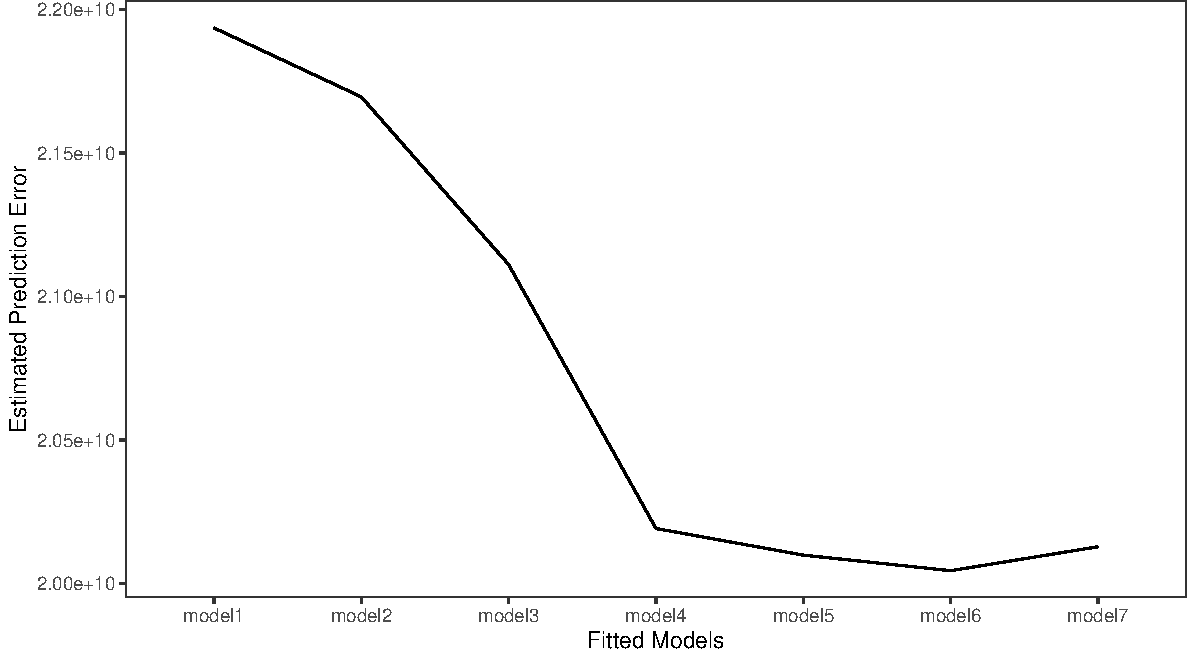
\includegraphics[scale=0.55]{Chapter3_codes_files/figure-latex/mse_plot_ch3-1.pdf}
\end{figure}

\noindent Model 5 explores adding more complexity to the data. We do it by adding four extra features: the square terms of bedrooms, bathrooms, latitude, and longitude. The prediction error continues decreasing. What about if we take out some of variables? In model 6 we take out  \texttt{lnbldg} (Log of building area in square feet) and  \texttt{dcbd} (Distance from the central business district) that are highly correlated with some of the other explanatory variables. Our prediction continues to improve.  Finally, what happens if we increase the order of the polynomial for longitude and latitude. The prediction error now gets slightly worse. Figure \ref{fig:mse_ch3} plots all of prediction errors for the previous 7 models.

There are a couple of lessons that we can take from this lab. First, as we add more complexity, the prediction error keeps getting smaller. Second, the choice of a model's complexity faces a bias/variance trade-off.  In future chapters, we will try to address and solve some of these questions.



\section{Simulation}


This section will set up a simulation exercise to illustrate the MSE
decomposition and bias/variance trade-off. We will simulate some data to
show the effects of omitting relevant, correlated, variables on bias and
variance.

Before diving into our simulations, we set a seed so the reader can
replicate our results and load the required packages:

\begin{Shaded}
\begin{Highlighting}[]
\KeywordTok{set.seed}\NormalTok{(}\DecValTok{101010}\NormalTok{) }\CommentTok{#set seeds}
\KeywordTok{require}\NormalTok{(}\StringTok{"dplyr"}\NormalTok{) }\CommentTok{#for data wrangling}
\KeywordTok{require}\NormalTok{(}\StringTok{"broom"}\NormalTok{) }\CommentTok{#transforms objects into tidy tables}
\KeywordTok{require}\NormalTok{(}\StringTok{"purrr"}\NormalTok{) }\CommentTok{#to generate simulations}
\end{Highlighting}
\end{Shaded}

In the simulation, the objective will be similar to the Lab, explain
house prices. However, in this simplified world, we know the true
functional relationship, house prices only depend on the number of
bedrooms and the number of bathrooms on the property:

\begin{align}\label{eq:true_f}
Price = 2 + 0.5 \times bedrooms+ 0.3 \times bathrooms
\end{align}

we can write this function in \texttt{R} as:

\begin{Shaded}
\begin{Highlighting}[]
\NormalTok{true_f<-}\StringTok{ }\ControlFlowTok{function}\NormalTok{(bedrooms,bathrooms)\{}
\NormalTok{  price<-}\StringTok{ }\DecValTok{2} \OperatorTok{+}\StringTok{ }\FloatTok{0.5}\OperatorTok{*}\NormalTok{bedrooms}\OperatorTok{+}\StringTok{ }\FloatTok{0.3}\OperatorTok{*}\NormalTok{bathrooms}
\NormalTok{  price}
\NormalTok{\}}
\end{Highlighting}
\end{Shaded}

The second step is to set up a function that will generate data based on
the true function, we will call it \texttt{dgp}. A key component for our
illustration is setting it up, so there is a correlation between
bedrooms and bathrooms. We set a correlation of \(\rho=0.7\) and sample
bedrooms from a Poisson distribution with parameter 4 that will give us
a discrete number of rooms. Bathrooms are a function of the number of
bedrooms plus a random Poisson component. Finally, the property price is
observed with an error that follows a standard normal and is
uncorrelated with the previous variables.

\begin{Shaded}
\begin{Highlighting}[]
\NormalTok{dgp<-}\ControlFlowTok{function}\NormalTok{(fx,sampleN)\{}
  \CommentTok{#arguments are the true data function (fx) }
  \CommentTok{#and the sample size (sampleN)}
  \CommentTok{#correlation between bedrooms and bathrooms is set to 0.7}
\NormalTok{  rho<-}\FloatTok{0.7} 
\NormalTok{  bedrooms<-}\KeywordTok{rpois}\NormalTok{(sampleN,}\DecValTok{3}\NormalTok{)  }
  \CommentTok{#sample bedrooms from a poisson distribution with mean and var 3}
\NormalTok{  bathrooms<-}\StringTok{ }\KeywordTok{floor}\NormalTok{(rho}\OperatorTok{*}\NormalTok{bedrooms }\OperatorTok{+}\StringTok{ }\KeywordTok{rpois}\NormalTok{(sampleN,}\DecValTok{1}\NormalTok{)) }
  \CommentTok{#bathrooms is correlated with bedrooms (floor function garanteed it is an integer)}
\NormalTok{  epsilon<-}\KeywordTok{rnorm}\NormalTok{(sampleN, }\DecValTok{0}\NormalTok{, }\DecValTok{1}\NormalTok{) }\CommentTok{#error term ~N(0,1)}
\NormalTok{  price<-}\StringTok{ }\KeywordTok{fx}\NormalTok{(bedrooms, bathrooms) }\OperatorTok{+}\StringTok{ }\NormalTok{epsilon}
\NormalTok{  tb <-}\StringTok{ }\KeywordTok{tibble}\NormalTok{(price,bedrooms,bathrooms) }\CommentTok{#return a tibble}
  \KeywordTok{return}\NormalTok{(tb)}
\NormalTok{\}}
\end{Highlighting}
\end{Shaded}

The function \texttt{dgp()} is then ready to take as arguments: a
function and a desired number of observations. This will return a table
with prices, bedrooms, and bathrooms. The third and final step is
generating simulated samples. The MSE equation:

\begin{equation}\label{eq:train_mse}
\underset{MSE\left(f(x_{0}),\hat{f}(x_{0})\right)}{\underbrace{E\left[\left(f(x_{0})-\hat{f}(x_{0})\right)^{2}\right]}}=\underbrace{\left(f(x_{0})-E\left[\hat{f}(x_{0})\right]\right)^{2}}_{\text{bias}^{2}\left(\hat{f}(x_{0})\right)}+\underbrace{E\left[\left(\hat{f}(x_{0})-E\left[\hat{f}(x_{0})\right]\right)^{2}\right]}_{\text{var}\left(\hat{f}(x_{0})\right)}
\end{equation}

\noindent tells us that the left side,
\(E[\left(f(x_{0})-\hat{f}(x_{0})\right)^{2}]\) is the average MSE that
we would get if we had a large number of samples and we fitted
\(f(x_0)\) to these sets. So we are going to generate 1,000 samples each
with 1,000 observations from our \texttt{dgp()} function and store it in
the \textbackslash{}texttt\{sim\_data\} element:

\begin{Shaded}
\begin{Highlighting}[]
\NormalTok{Obs<-}\DecValTok{1000}
\NormalTok{Nsimul<-}\DecValTok{1000}
\NormalTok{Nsim_list<-}\KeywordTok{as.list}\NormalTok{(}\KeywordTok{rep}\NormalTok{(Obs,Nsimul))}
\NormalTok{sim_data<-}\StringTok{ }\KeywordTok{tibble}\NormalTok{(}\DataTypeTok{sim_id=}\KeywordTok{seq}\NormalTok{(}\DecValTok{1}\NormalTok{,Nsimul),}\DataTypeTok{simulations=}\KeywordTok{lapply}\NormalTok{(Nsim_list,dgp, }\DataTypeTok{fx=}\NormalTok{true_f))}
\CommentTok{#The above line generates a data set that nests the simulations, }
\CommentTok{#each row is a table of 1,000 observations. }
\NormalTok{sim_data <-}\StringTok{ }\NormalTok{sim_data }\OperatorTok\StringTok{  }
\StringTok{     }\KeywordTok{mutate}\NormalTok{(}\DataTypeTok{fit1=} \KeywordTok{map}\NormalTok{(simulations,}\OperatorTok{~}\StringTok{ }\KeywordTok{lm}\NormalTok{(price}\OperatorTok{~}\DecValTok{1}\NormalTok{                    ,}\DataTypeTok{data=}\NormalTok{.x)),}
            \DataTypeTok{fit2=} \KeywordTok{map}\NormalTok{(simulations,}\OperatorTok{~}\StringTok{ }\KeywordTok{lm}\NormalTok{(price}\OperatorTok{~}\NormalTok{bedrooms             ,}\DataTypeTok{data=}\NormalTok{.x)),}
            \DataTypeTok{fit3=} \KeywordTok{map}\NormalTok{(simulations,}\OperatorTok{~}\StringTok{ }\KeywordTok{lm}\NormalTok{(price}\OperatorTok{~}\NormalTok{bedrooms}\OperatorTok{+}\NormalTok{bathrooms   ,}\DataTypeTok{data=}\NormalTok{.x))}
\NormalTok{            ) }\CommentTok{#fits our for models to each row and generates a new column}
\end{Highlighting}
\end{Shaded}

\noindent  For each of these samples, we are going to fit three models and evaluate them at a given point. We start by fitting a constant only model ($Y^1 =\beta_0$), then a model that only includes bathrooms ($Y^2=\beta_0 + \beta_1 bathrooms$), i.e.,
omits a relevant, correlated, variable. Finally, a model that includes all
the relevant variables ($Y^3=\beta_0 + \beta_1 bedrooms + \beta_2 bathrooms$). We evaluate the performance of the models choosing arbitrarily \(bed_0=3\) and \(bath_0 =1\). 

\begin{Shaded}
\begin{Highlighting}[]
\CommentTok{#Test values}
\NormalTok{bed_x0<-}\DecValTok{3}
\NormalTok{bath_x0<-}\DecValTok{1}
\CommentTok{#augment data with predictions}
\NormalTok{sim_data <-}\StringTok{ }\NormalTok{sim_data }\OperatorTok\StringTok{  }
\StringTok{     }\KeywordTok{mutate_at}\NormalTok{(}\DataTypeTok{.vars=}\KeywordTok{vars}\NormalTok{(}\KeywordTok{starts_with}\NormalTok{(}\StringTok{"fit"}\NormalTok{)),}\DataTypeTok{.funs=}\KeywordTok{list}\NormalTok{(}\ControlFlowTok{function}\NormalTok{(x)}
       \KeywordTok{map}\NormalTok{(x,augment,}\DataTypeTok{newdata=}\KeywordTok{tibble}\NormalTok{(}\DataTypeTok{bedrooms=}\NormalTok{bed_x0,}\DataTypeTok{bathrooms=}\NormalTok{bath_x0))))}
\end{Highlighting}
\end{Shaded}

\begin{figure}[H]
    \centering
    \caption{Simulated Fitted Values for Various Models}
    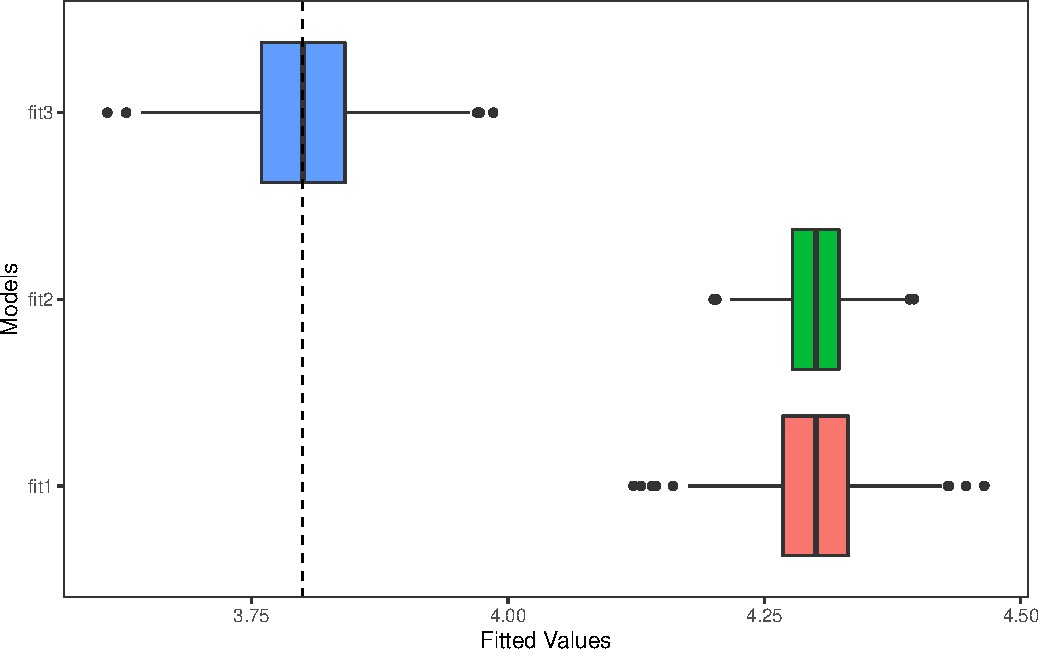
\includegraphics[scale=0.5]{Chapter3_codes_files/figure-latex/box_plots-1.pdf}
    \label{fig:simulation}
\end{figure}


\noindent Figure \ref{fig:simulation} shows the box plots of our fitted values,
for the three estimated models. The dashed black line marks the ``true''
value \$f(bed\_0,bath\_0)=\$3.8 and serves as ``target''. As expected, the first two models are biased. The third model is centered around the true value, showing us that it is unbiased. However, this third model has a wider interquartile range and whiskers, which is
less efficient than the other models.

From the simulations we then can calculate the bias, variance, and MSE for each
model:

\begin{Shaded}
\begin{Highlighting}[]
\NormalTok{sim_data<-}\StringTok{ }\NormalTok{sim_data}\OperatorTok\StringTok{ }\KeywordTok{mutate}\NormalTok{(}\DataTypeTok{true=}\KeywordTok{true_f}\NormalTok{(bed_x0,bath_x0)) }\CommentTok{#true value: "target"}
\NormalTok{sim_data<-}\StringTok{ }\NormalTok{sim_data}\OperatorTok\StringTok{ }\KeywordTok{group_by}\NormalTok{(model) }\OperatorTok\StringTok{ }\KeywordTok{mutate}\NormalTok{(}\DataTypeTok{bias=}\KeywordTok{mean}\NormalTok{(.fitted)}\OperatorTok{-}\NormalTok{true) }\CommentTok{#Bias}
\NormalTok{sim_data<-}\StringTok{ }\NormalTok{sim_data}\OperatorTok\StringTok{ }\KeywordTok{group_by}\NormalTok{(model) }\OperatorTok\StringTok{  }\KeywordTok{mutate}\NormalTok{(}\DataTypeTok{variance=}\NormalTok{(.fitted}\OperatorTok{-}\KeywordTok{mean}\NormalTok{(.fitted))}\OperatorTok{^}\DecValTok{2}\NormalTok{) }\CommentTok{#Variance}
\NormalTok{sim_data<-}\StringTok{ }\NormalTok{sim_data}\OperatorTok\StringTok{ }\KeywordTok{mutate}\NormalTok{(}\DataTypeTok{MSE=}\KeywordTok{mean}\NormalTok{((true}\OperatorTok{-}\NormalTok{.fitted ) }\OperatorTok{^}\StringTok{ }\DecValTok{2}\NormalTok{)) }\CommentTok{#MSE}

\NormalTok{results<-sim_data }\OperatorTok\StringTok{ }\KeywordTok{group_by}\NormalTok{(model) }\OperatorTok\StringTok{ }\KeywordTok{summarize}\NormalTok{(}\DataTypeTok{bias=}\KeywordTok{round}\NormalTok{(}\KeywordTok{mean}\NormalTok{(bias}\OperatorTok{^}\DecValTok{2}\NormalTok{),}\DecValTok{5}\NormalTok{),}
                                                             \DataTypeTok{variance=}\KeywordTok{round}\NormalTok{(}\KeywordTok{mean}\NormalTok{(variance),}\DecValTok{5}\NormalTok{),}
                                                             \DataTypeTok{MSE=}\KeywordTok{round}\NormalTok{(}\KeywordTok{mean}\NormalTok{(MSE),}\DecValTok{5}\NormalTok{))}
\NormalTok{results }\OperatorTok\StringTok{ }\KeywordTok{mutate}\NormalTok{(}\KeywordTok{all.equal}\NormalTok{(bias }\OperatorTok{+}\StringTok{ }\NormalTok{variance, MSE))}
\end{Highlighting}
\end{Shaded}

\begin{verbatim}
## # A tibble: 3 x 5
##   model  bias variance     MSE `all.equal(bias + variance, MSE)`
##   <fct> <dbl>    <dbl>   <dbl> <lgl>                            
## 1 fit1  0.250  0.00238 0.252   TRUE                             
## 2 fit2  0.250  0.00106 0.251   TRUE                             
## 3 fit3  0      0.00373 0.00373 TRUE
\end{verbatim}

This shows that the bias-variance decomposition holds for the fitted
values from these three models. Note also that the first two models are
biased. The third model is unbiased. However, it has a higher variance,
but the MSE is the smallest. This is why classical econometrics, through
unbiased estimation, solves the discussion of bias/variance trade-off.
Nevertheless, this requires knowing the ``true'' model. In future
chapters, we will see that the machine learning paradigm is willing to
accept some bias if that leads to reductions in the MSE.

The reader can easily adapt this simulation, and is encouraged, to see
what happens when the true model is a smaller one and a larger model is
estimated. Also is left as an exercise to extend the simulation and show
that  $Err(\hat{Y})>bias^{2}(\hat{f}(x_{0})+var(\hat{f}(x_{0})$.

